\documentclass[10pt,a4paper]{article}
\usepackage[a4paper,top=19mm,bottom=18mm,left=20mm,right=20mm,footskip=9mm]{geometry}
\usepackage{fontspec,xcolor,tikz,tcolorbox,tabularx,booktabs,enumitem,fancyhdr,microtype}
\usepackage{graphicx}
\special{dvipdfmx:config z 0}   % ohne Kompression, maximale Druckkompatibilitaet
\usetikzlibrary{arrows.meta,shadows.blur,fit}
\tcbuselibrary{skins}
\usepackage[ngerman,provide=*]{babel}
% Trennmuster wie beim Original-Build (dort fehlten die deutschen Muster,
% babel nahm die englischen). Ohne diese Zeile bricht Seite 2 anders um.
\babelprovide[hyphenrules=english]{ngerman}
\usepackage{hyperref}\hypersetup{hidelinks,pdftitle={Pending Orders – Kurz-Guide},pdfsubject={Buy Limit, Sell Limit, Buy Stop, Sell Stop}}

\setmainfont{IBMPlexSans-Regular.otf}[Path=../../fonts/,
  BoldFont={IBMPlexSans-SemiBold.otf}, ItalicFont={IBMPlexSans-Italic.otf},
  BoldItalicFont={IBMPlexSans-SemiBoldItalic.otf}]
\newfontfamily\light{IBMPlexSans-Light.otf}[Path=../../fonts/,
  BoldFont={IBMPlexSans-Regular.otf}, ItalicFont={IBMPlexSans-LightItalic.otf}]
\newfontfamily\mono{IBMPlexMono-Regular.otf}[Path=../../fonts/,
  BoldFont={IBMPlexMono-SemiBold.otf}]
\newcommand{\num}[1]{{\mono #1}}

% ---- Farben -------------------------------------------------------------
\definecolor{ink}{HTML}{14161A}    \definecolor{body}{HTML}{3C4249}
\definecolor{muted}{HTML}{6D757E}  \definecolor{soft}{HTML}{9AA1AA}
\definecolor{rule}{HTML}{E2E5E9}   \definecolor{greya}{HTML}{A8AEB6}
\definecolor{buy}{HTML}{0E7A4E}    \definecolor{sell}{HTML}{B23A2E}
\definecolor{buytint}{HTML}{E9F4EE} \definecolor{selltint}{HTML}{FAEDEB}
\definecolor{paper}{HTML}{F7F8F9}
\definecolor{pfbg}{HTML}{001328}\definecolor{pfgruen}{HTML}{0E7A4E}
\definecolor{pfgrau}{HTML}{97A5B4}\definecolor{pfrot}{HTML}{B23A2E}
\definecolor{pfgrey}{HTML}{6A6A6A}
\definecolor{wbg}{HTML}{0E2939} \definecolor{whead}{HTML}{0B2130} \definecolor{wfield}{HTML}{102B3C}
\definecolor{wborder}{HTML}{1D4256} \definecolor{waccent}{HTML}{1B6CA8} \definecolor{wgreen}{HTML}{3CB44A}
\definecolor{wtext}{HTML}{E7EEF2} \definecolor{wmuted}{HTML}{8FA6B3} \definecolor{wmark}{HTML}{3F88BD}
\definecolor{wdim}{HTML}{5F7A89} \definecolor{wtog}{HTML}{33505F} \definecolor{wknob}{HTML}{C3D2DA}
\definecolor{wred}{HTML}{E0524D} \definecolor{wchart}{HTML}{0B2030} \definecolor{wpill}{HTML}{5B6B76}
\definecolor{wtabtext}{HTML}{CDDBE3} \definecolor{wbadge}{HTML}{0B3A17}

% ---- Typografische Skala (1,25) -----------------------------------------
\newcommand{\display}{\light\fontsize{30}{34}\selectfont}
\newcommand{\hone}{\fontsize{19}{23}\selectfont\bfseries}
\newcommand{\htwo}{\fontsize{8}{11}\selectfont\bfseries}
\newcommand{\hthree}{\fontsize{12}{15}\selectfont\bfseries}
\newcommand{\leadf}{\light\fontsize{11.5}{17}\selectfont}
\renewcommand{\small}{\fontsize{8.6}{12.4}\selectfont}
\newcommand{\lbl}{\fontsize{7.6}{10}\selectfont}
\newcommand{\micro}{\fontsize{7}{9}\selectfont}
\newcommand{\wfont}{\fontsize{6.8}{8}\selectfont}
\newcommand{\wsmall}{\fontsize{5.8}{7}\selectfont}
\newcommand{\fine}{\fontsize{7.4}{9.2}\selectfont}
\newcommand{\foot}{\fontsize{6.2}{7.6}\selectfont}
\newcommand{\ls}{\addfontfeatures{LetterSpace=14}}
\newcommand{\lsx}{\addfontfeatures{LetterSpace=8}}
\normalsize\fontsize{9.4}{14}\selectfont
\color{body}\setlength{\parindent}{0pt}\setlength{\parskip}{0pt}
\setlength{\emergencystretch}{2em}
\hyphenpenalty=400\relax

% ---- Bausteine ----------------------------------------------------------
\newcommand{\kicker}[2]{{\htwo\ls\color{muted}\MakeUppercase{#2}\par}%
  \vspace{2mm}{\color{rule}\rule{\linewidth}{0.4pt}}\par\vspace{5.5mm}}
\newcommand{\Hone}[1]{{\hone\color{ink}#1\par}\vspace{3.5mm}}
\newcommand{\Htwo}[1]{{\htwo\ls\color{muted}\MakeUppercase{#1}\par}\vspace{4mm}}
\newcommand{\lead}[1]{{\leadf\color{body}\raggedright #1\par}}
\newcommand{\hr}{\par\vspace{7mm}{\color{rule}\rule{\linewidth}{0.4pt}}\par\vspace{6mm}}
\newcommand{\hd}[1]{{\micro\bfseries\ls\color{soft}\MakeUppercase{#1}}}
\tikzset{cnum/.style={circle,fill=ink,text=white,inner sep=0,minimum size=3.2mm,
  font=\bfseries\fontsize{5.6}{6}\selectfont}}
\newcommand{\cn}[1]{\tikz[baseline=-0.65ex]\node[cnum]{#1};}
\tikzset{pfnum/.style={circle,fill=ink,text=white,inner sep=0,minimum size=13,
  font=\bfseries\fontsize{7}{8}\selectfont}}
\newcommand{\pflab}{\fontsize{7}{8.5}\selectfont}
\newcommand{\pfn}[1]{\tikz[baseline=-0.7ex]\node[circle,fill=ink,text=white,inner sep=0,
  minimum size=4.4mm,font=\bfseries\fontsize{7}{8}\selectfont]{#1};}
\usetikzlibrary{calc}
% charts.tikz -- Vektor-Nachbau der vier Plattform-Chartbilder
% (img-pending-order-{bl,sl,bs,ss}.png, 174 x 96 px; Ursprung unten links,
% 1 Einheit = 1 px).  Je Bild 37 Rechtecke (Balken und Stiele), 2 Kreise
% (Kugeln: links rot = Kurs jetzt, rechts gruen = At price), 1 Dreieck
% (Richtung danach).  Farben: pfgruen, pfrot, pfgrau (abgedunkelte graue
% Kerzen fuer weissen Grund), definiert in der .tex.
%
% AUTOMATISCH ERZEUGT von tools/charts_aus_pdf.py aus
% originals/Pending-Orders-Guide_ORIGINAL.pdf (Seiten 1, 3, 4, 5).
% Alle Werte sind bitgenau aus dem Inhaltsstrom zurueckgerechnet.

\newcommand{\chartbl}{%
  \fill[pfrot] (14,66) rectangle (16.367,89.525);
  \fill[pfrot] (52.702,83.5) circle (3.651);
  \fill[pfrot] (51.497,44) rectangle (53.874,83.5);
  \fill[pfrot] (19,62) rectangle (21,85.624);
  \fill[pfrot] (23,58.683) rectangle (25.376,82);
  \fill[pfrot] (31,54.599) rectangle (33.502,78);
  \fill[pfrot] (39.251,49) rectangle (41.624,72.37);
  \fill[pfrot] (27,46.475) rectangle (29.367,70);
  \fill[pfrot] (35.125,46.375) rectangle (37.623,70);
  \fill[pfrot] (43.252,43.124) rectangle (45.75,66.75);
  \fill[pfrot] (47.371,38.251) rectangle (49.873,61.873);
  \fill[pfgrau] (64,39) rectangle (66,58.624);
  \fill[pfgrau] (55.498,38.251) rectangle (58,57.748);
  \fill[pfgrau] (68,36) rectangle (70,55.376);
  \fill[pfgrau] (76,36) rectangle (78.376,55.317);
  \fill[pfgrau] (59.655,33.37) rectangle (62,52.736);
  \fill[pfgrau] (88.251,32.63) rectangle (90.624,52);
  \fill[pfgrau] (80,31.699) rectangle (82.502,51);
  \fill[pfgrau] (72,30) rectangle (74.365,49.525);
  \fill[pfgrau] (96.37,29.251) rectangle (98.872,48.873);
  \fill[pfgrau] (104.498,31) rectangle (107,48.873);
  \fill[pfgrau] (84.125,28.375) rectangle (86.623,48);
  \fill[pfgrau] (92.251,27.849) rectangle (94.749,47);
  \fill[pfgrau] (100.498,23.604) rectangle (102.875,43);
  \fill[pfgruen] (152.349,83) -- (164.69,83) -- (158.476,89) -- cycle;
  \fill[pfgruen] (151.125,51.251) rectangle (153.623,70.876);
  \fill[pfgruen] (155.251,49) rectangle (157.624,68.159);
  \fill[pfgruen] (163.373,48) rectangle (165.875,69);
  \fill[pfgruen] (159.251,45) rectangle (161.749,64.151);
  \fill[pfgruen] (147,44) rectangle (149.502,63.401);
  \fill[pfgruen] (139,37.475) rectangle (141.365,57);
  \fill[pfgruen] (143,35) rectangle (145.376,54.422);
  \fill[pfgruen] (134,31.683) rectangle (136.376,51);
  \fill[pfgruen] (129.125,27) rectangle (131.502,46.158);
  \fill[pfgruen] (121,23.578) rectangle (123.376,43);
  \fill[pfgruen] (109.881,7.5) circle (3.594);
  \fill[pfgruen] (108.62,7.5) rectangle (111,38.962);
  \fill[pfgruen] (125,20.37) rectangle (127.345,39.736);
  \fill[pfgruen] (117,18) rectangle (119,37.376);
  \fill[pfgruen] (113,14.498) rectangle (115,34);
}
\newcommand{\chartsl}{%
  \fill[pfrot] (54,44) rectangle (56.376,63.422);
  \fill[pfrot] (67.493,15.5) circle (3.457);
  \fill[pfrot] (66.125,15.5) rectangle (68.625,60.962);
  \fill[pfrot] (58,41.599) rectangle (60.502,61);
  \fill[pfrot] (62.125,37.5) rectangle (64.502,57);
  \fill[pfrot] (50,36.624) rectangle (52,56);
  \fill[pfrot] (41.635,30) rectangle (44,49.525);
  \fill[pfrot] (46,27.624) rectangle (48,47);
  \fill[pfrot] (37,24.251) rectangle (39,43.875);
  \fill[pfrot] (32,19.376) rectangle (34,39);
  \fill[pfrot] (24,16.125) rectangle (26,35.749);
  \fill[pfrot] (11.373,13) rectangle (13.875,32.376);
  \fill[pfrot] (28,13) rectangle (30,32.502);
  \fill[pfrot] (19.635,10.475) rectangle (22,30);
  \fill[pfrot] (15.498,7.127) rectangle (18,26.748);
  \fill[pfrot] (152.282,18) -- (164.725,18) -- (158.5,11) -- cycle;
  \fill[pfgrau] (111.125,45) rectangle (113.502,64.158);
  \fill[pfgrau] (119.251,44) rectangle (121.749,63.501);
  \fill[pfgrau] (99,41.498) rectangle (101,61);
  \fill[pfgrau] (107,41.599) rectangle (109.502,61);
  \fill[pfgrau] (115.125,39) rectangle (117.623,58.625);
  \fill[pfgrau] (86.652,38.37) rectangle (89,57.63);
  \fill[pfgrau] (95,37.376) rectangle (97,57);
  \fill[pfgrau] (103,36) rectangle (105.376,55.317);
  \fill[pfgrau] (70.251,36.849) rectangle (72.749,54.501);
  \fill[pfgrau] (78.373,35) rectangle (80.875,54.376);
  \fill[pfgrau] (90.655,34.264) rectangle (93,53.63);
  \fill[pfgrau] (82.498,33.251) rectangle (85,52.873);
  \fill[pfgrau] (74.37,29.236) rectangle (76.748,48.866);
  \fill[pfgruen] (124.503,82.5) circle (3.465);
  \fill[pfgruen] (123.372,52.107) rectangle (125.75,82.5);
  \fill[pfgruen] (128.251,48) rectangle (130.749,71.75);
  \fill[pfgruen] (132.373,45) rectangle (134.749,68.158);
  \fill[pfgruen] (140.498,40.699) rectangle (143,64.301);
  \fill[pfgruen] (148.633,35) rectangle (151,58.525);
  \fill[pfgruen] (136.373,32.624) rectangle (138.875,56);
  \fill[pfgruen] (144.624,32.578) rectangle (147,56);
  \fill[pfgruen] (153,29.251) rectangle (155,52.875);
  \fill[pfgruen] (157,24.251) rectangle (159,48);
  \fill[pfgruen] (161,27.683) rectangle (163.356,43.736);
}
\newcommand{\chartbs}{%
  \fill[pfrot] (54,44) rectangle (56.376,63.422);
  \fill[pfrot] (67.493,15.5) circle (3.457);
  \fill[pfrot] (66.125,15.5) rectangle (68.625,60.962);
  \fill[pfrot] (58,41.599) rectangle (60.502,61);
  \fill[pfrot] (62.125,37.5) rectangle (64.502,57);
  \fill[pfrot] (50,36.624) rectangle (52,56);
  \fill[pfrot] (41.635,30) rectangle (44,49.525);
  \fill[pfrot] (46,27.624) rectangle (48,47);
  \fill[pfrot] (37,24.251) rectangle (39,43.875);
  \fill[pfrot] (32,19.376) rectangle (34,39);
  \fill[pfrot] (24,16.125) rectangle (26,35.749);
  \fill[pfrot] (11.373,13) rectangle (13.875,32.376);
  \fill[pfrot] (28,13) rectangle (30,32.502);
  \fill[pfrot] (19.635,10.475) rectangle (22,30);
  \fill[pfrot] (15.498,7.127) rectangle (18,26.748);
  \fill[pfgrau] (111.125,39) rectangle (113.502,58.5);
  \fill[pfgrau] (119.251,38.248) rectangle (121.749,57.75);
  \fill[pfgrau] (99,36) rectangle (101,55.376);
  \fill[pfgrau] (107,36) rectangle (109.502,55.301);
  \fill[pfgrau] (115.125,33.251) rectangle (117.623,52.876);
  \fill[pfgrau] (86.624,32.578) rectangle (89,52);
  \fill[pfgrau] (95,31.624) rectangle (97,51);
  \fill[pfgrau] (103,30) rectangle (105.365,49.525);
  \fill[pfgrau] (70.249,31) rectangle (72.747,48.874);
  \fill[pfgrau] (78.37,29.251) rectangle (80.872,48.873);
  \fill[pfgrau] (90.635,28.475) rectangle (93,48);
  \fill[pfgrau] (82.498,27.699) rectangle (85,47);
  \fill[pfgrau] (74.373,23.632) rectangle (76.749,43);
  \fill[pfgruen] (161,66) rectangle (163.367,89.525);
  \fill[pfgruen] (124.5,83.5) circle (3.476);
  \fill[pfgruen] (123.372,43.107) rectangle (125.75,83.5);
  \fill[pfgruen] (156,62) rectangle (158.502,85.498);
  \fill[pfgruen] (152,58.683) rectangle (154.376,82);
  \fill[pfgruen] (144,54.498) rectangle (146,78);
  \fill[pfgruen] (135.624,49) rectangle (138,72.422);
  \fill[pfgruen] (140,46.376) rectangle (142,70);
  \fill[pfgruen] (148,46.376) rectangle (150,70);
  \fill[pfgruen] (131.498,43.127) rectangle (134,66.748);
  \fill[pfgruen] (127.371,38.251) rectangle (129.873,61.873);
  \fill[pfgruen] (152.427,12) -- (164.557,12) -- (158.459,18) -- cycle;
}
\newcommand{\chartss}{%
  \fill[pfrot] (14,66) rectangle (16.367,89.525);
  \fill[pfrot] (152.302,89) -- (164.651,89) -- (158.5,82) -- cycle;
  \fill[pfrot] (52.702,83.5) circle (3.651);
  \fill[pfrot] (51.497,44) rectangle (53.874,83.5);
  \fill[pfrot] (19,62) rectangle (21,85.624);
  \fill[pfrot] (23,58.683) rectangle (25.376,82);
  \fill[pfrot] (31,54.599) rectangle (33.502,78);
  \fill[pfrot] (39.251,49) rectangle (41.624,72.37);
  \fill[pfrot] (27,46.475) rectangle (29.367,70);
  \fill[pfrot] (35.125,46.375) rectangle (37.623,70);
  \fill[pfrot] (43.252,43.124) rectangle (45.75,66.75);
  \fill[pfrot] (47.371,38.251) rectangle (49.873,61.873);
  \fill[pfgrau] (64,39) rectangle (66,58.624);
  \fill[pfgrau] (55.498,38.251) rectangle (58,57.748);
  \fill[pfgrau] (68,36) rectangle (70,55.376);
  \fill[pfgrau] (76,36) rectangle (78.376,55.317);
  \fill[pfgrau] (59.655,33.37) rectangle (62,52.736);
  \fill[pfgrau] (88.251,32.63) rectangle (90.624,52);
  \fill[pfgrau] (80,31.699) rectangle (82.502,51);
  \fill[pfgrau] (72,30) rectangle (74.365,49.525);
  \fill[pfgrau] (96.37,29.251) rectangle (98.872,48.873);
  \fill[pfgrau] (104.498,31) rectangle (107,48.873);
  \fill[pfgrau] (84.125,28.375) rectangle (86.623,48);
  \fill[pfgrau] (92.251,27.849) rectangle (94.749,47);
  \fill[pfgrau] (100.498,23.604) rectangle (102.875,43);
  \fill[pfgruen] (121,44) rectangle (123.376,63.422);
  \fill[pfgruen] (109.882,15.5) circle (3.571);
  \fill[pfgruen] (108.621,15.5) rectangle (111,60.95);
  \fill[pfgruen] (117,41.498) rectangle (119,61);
  \fill[pfgruen] (113,37.376) rectangle (115,57);
  \fill[pfgruen] (125,36.683) rectangle (127.376,56);
  \fill[pfgruen] (133.125,30) rectangle (135.623,49.625);
  \fill[pfgruen] (129.125,27.842) rectangle (131.502,47);
  \fill[pfgruen] (138,24.251) rectangle (140.502,43.873);
  \fill[pfgruen] (143,19.475) rectangle (145.365,39);
  \fill[pfgruen] (151.128,16.124) rectangle (153.626,35.75);
  \fill[pfgruen] (147,13) rectangle (149.502,32.401);
  \fill[pfgruen] (163.373,13) rectangle (165.875,32.376);
  \fill[pfgruen] (155.252,10.395) rectangle (157.623,30);
  \fill[pfgruen] (159.252,7.124) rectangle (161.751,26.75);
}

% Mini-Fassungen (Spickzettel S. 5, Deckblatt).
% Im ORIGINAL-PDF sind sie geometrisch und farblich identisch mit den
% grossen Fassungen (nur kleiner skaliert) -> Verweis statt Kopie.
\newcommand{\chartblmini}{\chartbl}
\newcommand{\chartslmini}{\chartsl}
\newcommand{\chartbsmini}{\chartbs}
\newcommand{\chartssmini}{\chartss}

% weicher Schatten fuer eingebundene Grafiken
\tikzset{softshadow/.style={blur shadow={shadow blur steps=16,shadow xshift=0pt,
  shadow yshift=-0.9pt,shadow opacity=30,shadow blur radius=1.5mm}}}
\newcommand{\shadowfig}[2][80mm]{%
  \tikz[baseline=(current bounding box.north)]\node[inner sep=0,softshadow]
    {\includegraphics[width=#1]{#2}};}

\newtcolorbox{merk}{enhanced,colback=paper,colframe=paper,boxrule=0pt,arc=0pt,
  borderline west={2pt}{0pt}{ink},left=5mm,right=5mm,top=3.5mm,bottom=3.5mm,boxsep=0pt,
  before skip=6mm,after skip=0pt,fontupper=\small\color{body}}
\newtcolorbox{prule}[1]{enhanced,colback=white,colframe=rule,boxrule=0.4pt,arc=1mm,
  borderline west={2pt}{0pt}{#1},left=4mm,right=4mm,top=2.6mm,bottom=2.6mm,boxsep=0pt,
  before skip=2.2mm,after skip=0pt,fontupper=\small\color{body}}
\newtcolorbox{soft}{enhanced,colback=paper,colframe=paper,boxrule=0pt,arc=1.5mm,
  left=5mm,right=5mm,top=4mm,bottom=4mm,boxsep=0pt,before skip=0pt,after skip=0pt,
  before upper={\raggedright\hyphenpenalty=10000\relax\exhyphenpenalty=10000\relax}}

\pagestyle{fancy}\fancyhf{}\renewcommand{\headrulewidth}{0pt}

\fancyfoot[L]{\micro\color{soft}\ls PENDING ORDERS · STANDARD TIER}
\begin{document}
% ==== DECKBLATT (Test): Hintergrund cover-bg.pdf, Inhalte absolut in mm ====
% Platzhalter-Koordinaten aus cover.svg (y von oben, hier negativ). Baselines:
% Versalhoehe (0,698 em) mittig in der Platzhalter-Box; Kicker oben buendig
% auf 20,5 mm (gleiche Starthoehe wie die Innenseiten).
% Charts: linke Kante des Chart-Inhalts buendig mit der Textkante (x=20 bzw. 117,5).
% Abgezogen wird die linke Inhaltskante aus charts.tikz (bs/sl: 11.373, bl/ss: 14 px);
% bei Aenderungen an charts.tikz diese Werte anpassen.
\definecolor{cvkicker}{HTML}{9FB3C2}\definecolor{cvsub}{HTML}{D5DEE6}
\definecolor{cvpill}{HTML}{5E7F95}\definecolor{cvpilltext}{HTML}{C9D6E0}
\thispagestyle{empty}
\noindent\begin{tikzpicture}[remember picture,overlay,x=1mm,y=1mm,every node/.style={outer sep=0pt}]
\begin{scope}[shift={(current page.north west)}]
\node[anchor=north west,inner sep=0] at (0,0) {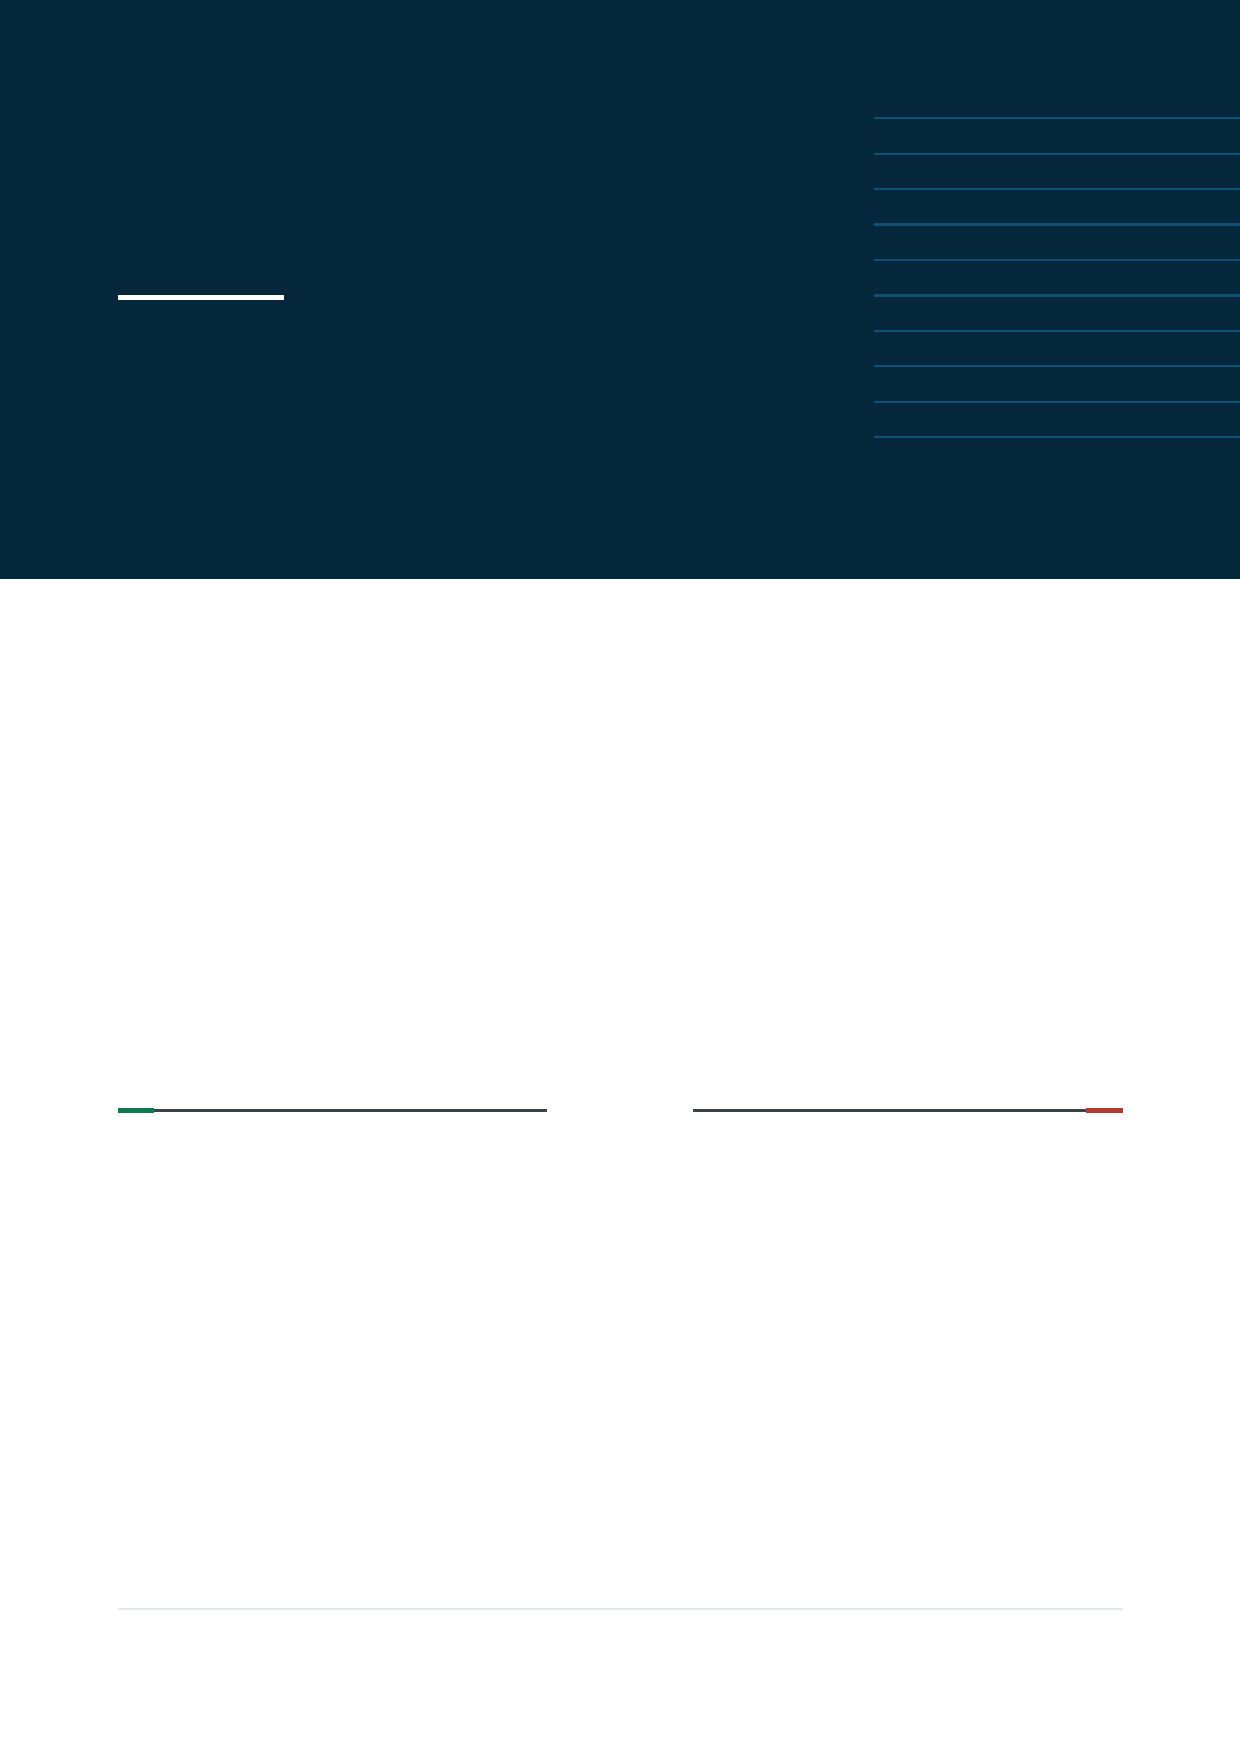
\includegraphics[width=210mm,height=297mm]{cover-bg.pdf}};
\node[anchor=base west,inner sep=0,text=cvkicker,font=\htwo\ls] at (20,-22.463) {TRADING-GRUNDLAGEN};
\node[anchor=base west,inner sep=0,text=white,font=\display] at (20,-41.18) {Pending Orders};
\node[anchor=base west,inner sep=0,text=cvsub] at (20,-60.673) {\parbox[t]{124mm}{\leadf\raggedright Die vier Ordertypen auf einen Blick – damit du Einstieg, Auslösepreis und Richtung richtig kombinierst.\par}};
\draw[cvpill,line width=0.4pt,rounded corners=1.6mm] (20,-75) rectangle (98,-81.5);
\node[anchor=base,inner sep=0,text=cvpilltext,font=\micro\bfseries\ls] at (59,-79.109) {4 ORDERTYPEN. 1 KLARE ENTSCHEIDUNGSLOGIK.};
\node[anchor=base,inner sep=0,text=muted,font=\lbl\bfseries\ls] at (105,-115.932) {AT PRICE ÜBER DEM AKTUELLEN KURS};
\node[anchor=base,inner sep=0,text=ink,font=\lbl\bfseries\ls] at (105,-188.932) {KURS JETZT};
\node[anchor=base,inner sep=0,text=muted,font=\lbl\bfseries\ls] at (105,-260.932) {AT PRICE UNTER DEM AKTUELLEN KURS};
\begin{scope}[shift={(20-11.373*72.5/174,-163)},scale=72.5/174] \chartbsmini \end{scope}
\node[anchor=base west,inner sep=0,text=buy,font=\hthree] at (20,-171.472) {BUY STOP};
\node[anchor=base west,inner sep=0,text=muted,font=\small] at (20,-177.305) {Ausbruch nach oben};
\begin{scope}[shift={(117.5-11.373*72.5/174,-163)},scale=72.5/174] \chartslmini \end{scope}
\node[anchor=base west,inner sep=0,text=sell,font=\hthree] at (117.5,-171.472) {SELL LIMIT};
\node[anchor=base west,inner sep=0,text=muted,font=\small] at (117.5,-177.305) {teurer verkaufen};
\begin{scope}[shift={(20-14*72.5/174,-252)},scale=72.5/174] \chartblmini \end{scope}
\node[anchor=base west,inner sep=0,text=buy,font=\hthree] at (20,-200.972) {BUY LIMIT};
\node[anchor=base west,inner sep=0,text=muted,font=\small] at (20,-206.805) {günstiger kaufen};
\begin{scope}[shift={(117.5-14*72.5/174,-252)},scale=72.5/174] \chartssmini \end{scope}
\node[anchor=base west,inner sep=0,text=sell,font=\hthree] at (117.5,-200.972) {SELL STOP};
\node[anchor=base west,inner sep=0,text=muted,font=\small] at (117.5,-206.805) {Ausbruch nach unten};
\node[anchor=base west,inner sep=0,text=soft,font=\micro\ls] at (20,-277.359) {PENDING ORDERS};
\node[anchor=base east,inner sep=0,text=soft,font=\micro\ls] at (190,-277.359) {STANDARD TIER};
\end{scope}
\end{tikzpicture}
\clearpage
\kicker{}{Fundament}
\Hone{Was eine Pending Order ist}
\begin{minipage}{128mm}\lead{Du kaufst oder verkaufst nicht sofort. Du legst vorher einen Kurs fest –
und die Plattform wartet für dich, bis er erreicht ist.}\end{minipage}
\par\vspace{8mm}
\noindent\begin{minipage}[t]{82mm}\vspace{0pt}\begin{soft}
{\htwo\ls\color{muted}NEW MARKET ORDER}\par\vspace{2mm}
{\hthree\color{ink}Sofort.}\par\vspace{1.5mm}
{\color{body}Du klickst – und der Kauf oder Verkauf passiert im selben Moment,
zum Kurs, der gerade gilt.}\end{soft}\end{minipage}\hfill
\begin{minipage}[t]{82mm}\vspace{0pt}\begin{soft}
{\htwo\ls\color{muted}NEW PENDING ORDER}\par\vspace{2mm}
{\hthree\color{ink}Später.}\par\vspace{1.5mm}
{\color{body}Du trägst bei At price deinen Aktivierungspunkt ein. Erreicht der Markt ihn,
wird die Order ausgelöst.}\end{soft}\end{minipage}
\hr
\Htwo{Der aktuelle Kurs ist dein Nullpunkt}
{\color{body}Jeder Wert, den du bei At price einträgst, liegt entweder über oder unter dem Kurs
von jetzt. Genau daran erkennst du, welchen Ordertyp du brauchst.}\par\vspace{6mm}
\noindent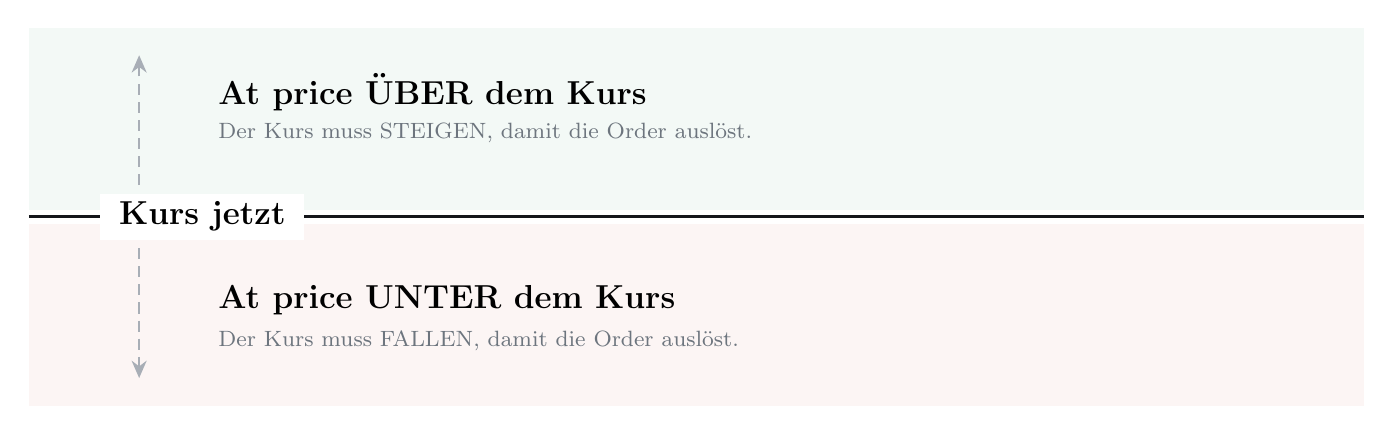
\begin{tikzpicture}[x=1mm,y=1mm,font=\lbl]
\fill[buytint,opacity=0.55] (0,0.9) rectangle (169.5,24.0);
\fill[selltint,opacity=0.55] (0,-24.0) rectangle (169.5,-0.9);
\draw[ink,line width=0.9pt] (0,0) -- (169.5,0);
\node[anchor=west,inner sep=0,font=\hthree] at (9,0) {\colorbox{white}{\;Kurs jetzt\;}};
\draw[greya,line width=0.8pt,dash pattern=on 1.4mm off 0.9mm,-{Stealth[length=2.2mm,width=1.9mm]}] (14,4) -- (14,20.5);
\node[anchor=west,inner sep=0,font=\hthree] at (24,15.8) {At price ÜBER dem Kurs};
\node[anchor=west,inner sep=0,text=muted] at (24,10.600000000000001) {Der Kurs muss STEIGEN, damit die Order auslöst.}; 
\draw[greya,line width=0.8pt,dash pattern=on 1.4mm off 0.9mm,-{Stealth[length=2.2mm,width=1.9mm]}] (14,-4) -- (14,-20.5);
\node[anchor=west,inner sep=0,font=\hthree] at (24,-10.600000000000001) {At price UNTER dem Kurs};
\node[anchor=west,inner sep=0,text=muted] at (24,-15.8) {Der Kurs muss FALLEN, damit die Order auslöst.}; 
\end{tikzpicture}
\par\vspace{4mm}
{\color{muted}\small Kaufen und unter dem Kurs: \textcolor{buy}{\bfseries Buy Limit}.
Kaufen und über dem Kurs: \textcolor{buy}{\bfseries Buy Stop}.
Verkaufen und über dem Kurs: \textcolor{sell}{\bfseries Sell Limit}.
Verkaufen und unter dem Kurs: \textcolor{sell}{\bfseries Sell Stop}.}
\hr
\Htwo{Warum im Voraus planen}
\noindent\begin{minipage}[t]{53mm}\vspace{0pt}\raggedright
{\bfseries Du musst nicht am Bildschirm sitzen.}\par\vspace{1mm}
{\color{muted}\small Die Plattform wartet für dich – auch nachts oder während du arbeitest.}
\end{minipage}\hfill
\begin{minipage}[t]{53mm}\vspace{0pt}\raggedright
{\bfseries Du entscheidest in Ruhe.}\par\vspace{1mm}
{\color{muted}\small Den Kurs legst du vorher fest – nicht in dem Moment, in dem sich der Markt bewegt.}
\end{minipage}\hfill
\begin{minipage}[t]{53mm}\vspace{0pt}\raggedright
{\bfseries Sie löst nur bei deinem Wert aus.}\par\vspace{1mm}
{\color{muted}\small Nicht früher. Du läufst dem Kurs nicht hinterher.}
\end{minipage}
\clearpage
\kicker{}{Die Limit-Typen}
\Hone{Limit wartet auf den besseren Kurs}
\begin{minipage}{125mm}\lead{Bei Limit liegt dein At-price-Wert dort, wo du einen günstigeren
Preis bekommst als jetzt. Erreicht der Markt deinen Aktivierungspunkt, wird die Order ausgelöst.}\end{minipage}
\par\vspace{10mm}

{\hthree\color{buy}BUY LIMIT}\hfill
{\fine\color{muted}günstiger kaufen · At price liegt unter dem Kurs}\par\vspace{1.4mm}
{\color{rule}\rule{\linewidth}{0.4pt}}\par\vspace{5mm}
\noindent\begin{minipage}[t]{94mm}\vspace{0pt}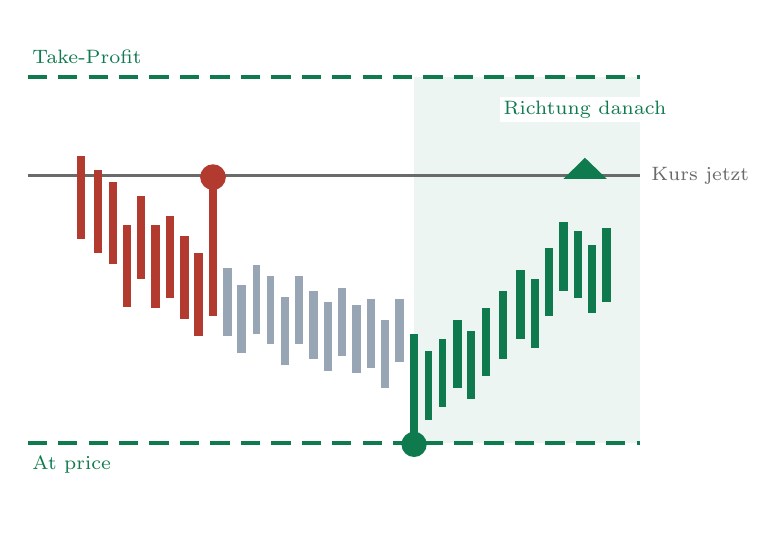
\begin{tikzpicture}[x=0.44660mm,y=0.44660mm]
\useasboundingbox (0,-10) rectangle (206,126);
\fill[pfgruen,opacity=0.08] (110,8) rectangle (174,112);
\draw[pfgruen,line width=1.5,dash pattern=on 7 off 4] (0,112) -- (174,112);
\node[anchor=south west,inner sep=1.5,fill=white,text=pfgruen] at (0,114.5) {\pflab Take-Profit};
\draw[pfgruen,line width=1.5,dash pattern=on 7 off 4] (0,8) -- (174,8);
\node[anchor=north west,inner sep=1.5,fill=white,text=pfgruen] at (0,5.5) {\pflab At price};
\draw[pfgrey,line width=0.9] (0,84) -- (174,84);
\node[anchor=west,inner sep=1.5,fill=white,text=pfgrey] at (176,84) {\pflab Kurs jetzt};
\chartbl
\node[anchor=south,inner sep=1.5,fill=white,text=pfgruen] at (158.5,99) {\pflab Richtung danach};
\end{tikzpicture}\end{minipage}\hfill
\begin{minipage}[t]{72mm}\vspace{1mm}\raggedright
{\bfseries\color{ink}Kurs jetzt}\par{\color{muted}\small Die graue Linie ist der Kurs in dem Moment, in dem du die Order aufgibst. Die rote Kugel zeigt genau diesen Punkt.}\par\vspace{3.8mm}
{\bfseries\color{pfgruen}At price}\par{\color{muted}\small Dein Aktivierungspunkt, hier \textbf{unter} dem Kurs. Erreicht der Markt ihn, wird die Order ausgelöst. Bis dahin passiert nichts.}\par\vspace{3.8mm}
{\bfseries\color{pfgruen}Richtung danach}\par{\color{muted}\small Das Dreieck zeigt, wohin es dann gehen soll: der Kurs soll \textbf{steigen} – bis zu deinem Take-Profit.}\par\vspace{3.8mm}
{\bfseries\color{ink}Wann sinnvoll}\par{\color{muted}\small Wenn du glaubst, der Kurs fällt kurz zurück, bevor er steigt. Du kaufst dann günstiger als jetzt.}
\end{minipage}\par
\hr

{\hthree\color{sell}SELL LIMIT}\hfill
{\fine\color{muted}teurer verkaufen · At price liegt über dem Kurs}\par\vspace{1.4mm}
{\color{rule}\rule{\linewidth}{0.4pt}}\par\vspace{5mm}
\noindent\begin{minipage}[t]{94mm}\vspace{0pt}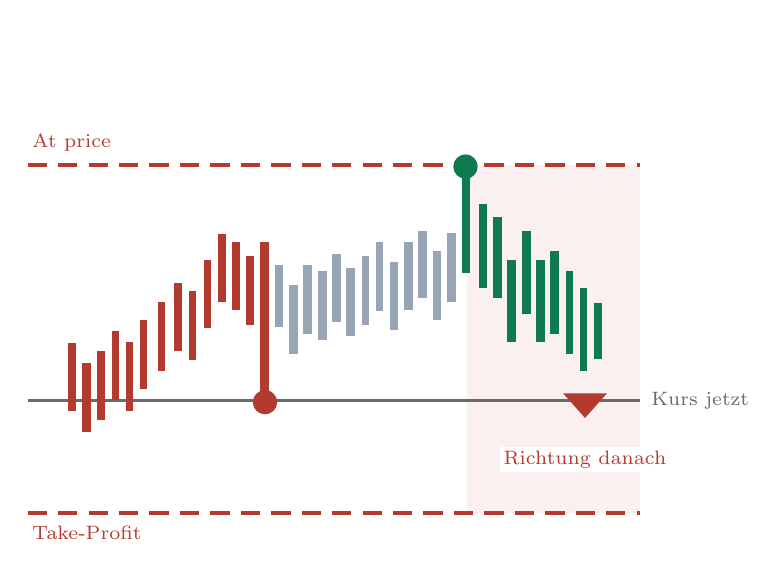
\begin{tikzpicture}[x=0.44660mm,y=0.44660mm]
\useasboundingbox (0,-26) rectangle (206,122);
\fill[pfrot,opacity=0.08] (125,-16) rectangle (174,83);
\draw[pfrot,line width=1.5,dash pattern=on 7 off 4] (0,-16) -- (174,-16);
\node[anchor=north west,inner sep=1.5,fill=white,text=pfrot] at (0,-18.5) {\pflab Take-Profit};
\draw[pfrot,line width=1.5,dash pattern=on 7 off 4] (0,83) -- (174,83);
\node[anchor=south west,inner sep=1.5,fill=white,text=pfrot] at (0,85.5) {\pflab At price};
\draw[pfgrey,line width=0.9] (0,16) -- (174,16);
\node[anchor=west,inner sep=1.5,fill=white,text=pfgrey] at (176,16) {\pflab Kurs jetzt};
\chartsl
\node[anchor=north,inner sep=1.5,fill=white,text=pfrot] at (158.5,3) {\pflab Richtung danach};
\end{tikzpicture}\end{minipage}\hfill
\begin{minipage}[t]{72mm}\vspace{1mm}\raggedright
{\bfseries\color{ink}Kurs jetzt}\par{\color{muted}\small Die graue Linie ist der Kurs in dem Moment, in dem du die Order aufgibst. Die rote Kugel zeigt genau diesen Punkt.}\par\vspace{3.8mm}
{\bfseries\color{pfrot}At price}\par{\color{muted}\small Dein Aktivierungspunkt, hier \textbf{über} dem Kurs. Erreicht der Markt ihn, wird die Order ausgelöst. Bis dahin passiert nichts.}\par\vspace{3.8mm}
{\bfseries\color{pfrot}Richtung danach}\par{\color{muted}\small Das Dreieck zeigt, wohin es dann gehen soll: der Kurs soll \textbf{fallen} – bis zu deinem Take-Profit.}\par\vspace{3.8mm}
{\bfseries\color{ink}Wann sinnvoll}\par{\color{muted}\small Wenn du glaubst, der Kurs steigt noch ein Stück, bevor er fällt. Du verkaufst dann teurer als jetzt.}
\end{minipage}\par
\clearpage
\kicker{}{Die Stop-Typen}
\Hone{Stop wartet auf die Bewegung}
\begin{minipage}{125mm}\lead{Bei Stop liegt dein At-price-Wert auf der ungünstigeren Seite.
Die Order löst erst aus, wenn der Kurs durch den Wert bricht – du steigst also erst ein, wenn
die Bewegung schon da ist.}\end{minipage}
\par\vspace{10mm}

{\hthree\color{buy}BUY STOP}\hfill
{\fine\color{muted}Ausbruch nach oben kaufen · At price liegt über dem Kurs}\par\vspace{1.4mm}
{\color{rule}\rule{\linewidth}{0.4pt}}\par\vspace{5mm}
\noindent\begin{minipage}[t]{94mm}\vspace{0pt}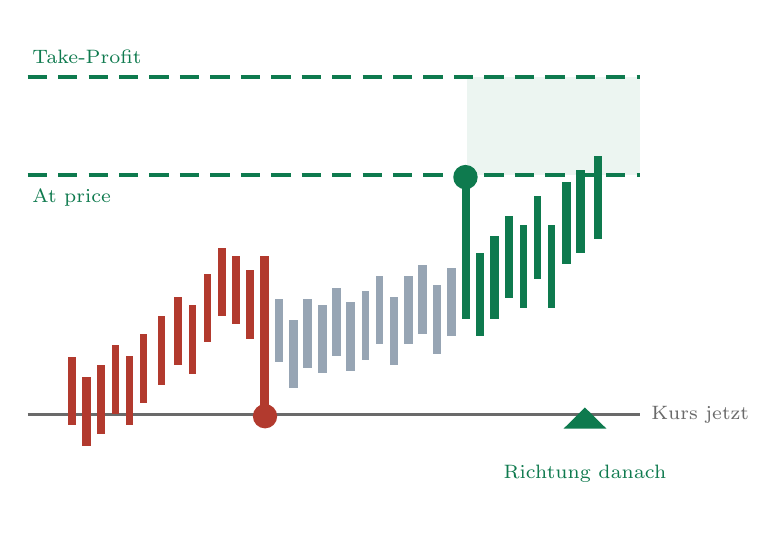
\begin{tikzpicture}[x=0.44660mm,y=0.44660mm]
\useasboundingbox (0,-10) rectangle (206,126);
\fill[pfgruen,opacity=0.08] (125,84) rectangle (174,112);
\draw[pfgruen,line width=1.5,dash pattern=on 7 off 4] (0,112) -- (174,112);
\node[anchor=south west,inner sep=1.5,fill=white,text=pfgruen] at (0,114.5) {\pflab Take-Profit};
\draw[pfgruen,line width=1.5,dash pattern=on 7 off 4] (0,84) -- (174,84);
\node[anchor=north west,inner sep=1.5,fill=white,text=pfgruen] at (0,81.5) {\pflab At price};
\draw[pfgrey,line width=0.9] (0,16) -- (174,16);
\node[anchor=west,inner sep=1.5,fill=white,text=pfgrey] at (176,16) {\pflab Kurs jetzt};
\chartbs
\node[anchor=north,inner sep=1.5,fill=white,text=pfgruen] at (158.5,3) {\pflab Richtung danach};
\end{tikzpicture}\end{minipage}\hfill
\begin{minipage}[t]{72mm}\vspace{1mm}\raggedright
{\bfseries\color{ink}Kurs jetzt}\par{\color{muted}\small Die graue Linie ist der Kurs in dem Moment, in dem du die Order aufgibst. Die rote Kugel zeigt genau diesen Punkt.}\par\vspace{3.8mm}
{\bfseries\color{pfgruen}At price}\par{\color{muted}\small Dein Aktivierungspunkt, hier \textbf{über} dem Kurs. Erreicht der Markt ihn, wird die Order ausgelöst. Bis dahin passiert nichts.}\par\vspace{3.8mm}
{\bfseries\color{pfgruen}Richtung danach}\par{\color{muted}\small Das Dreieck zeigt, wohin es dann gehen soll: der Kurs soll \textbf{steigen} – bis zu deinem Take-Profit.}\par\vspace{3.8mm}
{\bfseries\color{ink}Wann sinnvoll}\par{\color{muted}\small Wenn du erst kaufen willst, sobald der Kurs eine Hürde nach oben genommen hat – nicht vorher.}
\end{minipage}\par
\hr

{\hthree\color{sell}SELL STOP}\hfill
{\fine\color{muted}Ausbruch nach unten verkaufen · At price liegt unter dem Kurs}\par\vspace{1.4mm}
{\color{rule}\rule{\linewidth}{0.4pt}}\par\vspace{5mm}
\noindent\begin{minipage}[t]{94mm}\vspace{0pt}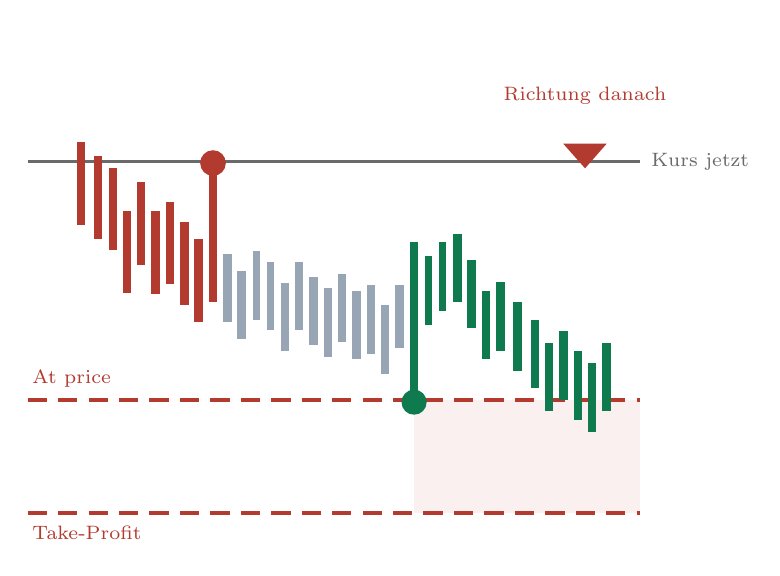
\begin{tikzpicture}[x=0.44660mm,y=0.44660mm]
\useasboundingbox (0,-26) rectangle (206,122);
\fill[pfrot,opacity=0.08] (110,-16) rectangle (174,16);
\draw[pfrot,line width=1.5,dash pattern=on 7 off 4] (0,-16) -- (174,-16);
\node[anchor=north west,inner sep=1.5,fill=white,text=pfrot] at (0,-18.5) {\pflab Take-Profit};
\draw[pfrot,line width=1.5,dash pattern=on 7 off 4] (0,16) -- (174,16);
\node[anchor=south west,inner sep=1.5,fill=white,text=pfrot] at (0,18.5) {\pflab At price};
\draw[pfgrey,line width=0.9] (0,84) -- (174,84);
\node[anchor=west,inner sep=1.5,fill=white,text=pfgrey] at (176,84) {\pflab Kurs jetzt};
\chartss
\node[anchor=south,inner sep=1.5,fill=white,text=pfrot] at (158.5,99) {\pflab Richtung danach};
\end{tikzpicture}\end{minipage}\hfill
\begin{minipage}[t]{72mm}\vspace{1mm}\raggedright
{\bfseries\color{ink}Kurs jetzt}\par{\color{muted}\small Die graue Linie ist der Kurs in dem Moment, in dem du die Order aufgibst. Die rote Kugel zeigt genau diesen Punkt.}\par\vspace{3.8mm}
{\bfseries\color{pfrot}At price}\par{\color{muted}\small Dein Aktivierungspunkt, hier \textbf{unter} dem Kurs. Erreicht der Markt ihn, wird die Order ausgelöst. Bis dahin passiert nichts.}\par\vspace{3.8mm}
{\bfseries\color{pfrot}Richtung danach}\par{\color{muted}\small Das Dreieck zeigt, wohin es dann gehen soll: der Kurs soll \textbf{fallen} – bis zu deinem Take-Profit.}\par\vspace{3.8mm}
{\bfseries\color{ink}Wann sinnvoll}\par{\color{muted}\small Wenn du erst verkaufen willst, sobald der Kurs nach unten durchbricht – nicht vorher.}
\end{minipage}\par
\clearpage
\kicker{}{Spickzettel}
\Hone{Alle vier nebeneinander}
\begin{minipage}{128mm}\lead{Vier Bilder, ein Muster: Die rote Kugel ist der Kurs, wenn du die Order
aufgibst. Die grüne Kugel ist dein At price. Das Dreieck zeigt, wohin es danach gehen soll.}\end{minipage}
\par\vspace{11mm}
\noindent\hspace*{-1mm}\begin{minipage}[t]{40mm}\vspace{0pt}\centering
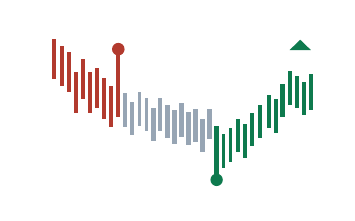
\begin{tikzpicture}[x=0.21839mm,y=0.21839mm]\useasboundingbox (0,0) rectangle (174.0,96.0);\chartblmini\end{tikzpicture}\par\vspace{2.4mm}
{\color{buy}\bfseries\lbl BUY LIMIT}
\end{minipage}\hfill
\begin{minipage}[t]{40mm}\vspace{0pt}\centering
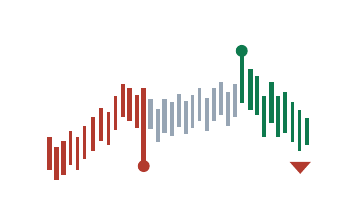
\begin{tikzpicture}[x=0.21839mm,y=0.21839mm]\useasboundingbox (0,0) rectangle (174.0,96.0);\chartslmini\end{tikzpicture}\par\vspace{2.4mm}
{\color{sell}\bfseries\lbl SELL LIMIT}
\end{minipage}\hfill
\begin{minipage}[t]{40mm}\vspace{0pt}\centering
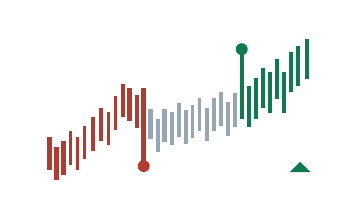
\begin{tikzpicture}[x=0.21839mm,y=0.21839mm]\useasboundingbox (0,0) rectangle (174.0,96.0);\chartbsmini\end{tikzpicture}\par\vspace{2.4mm}
{\color{buy}\bfseries\lbl BUY STOP}
\end{minipage}\hfill
\begin{minipage}[t]{40mm}\vspace{0pt}\centering
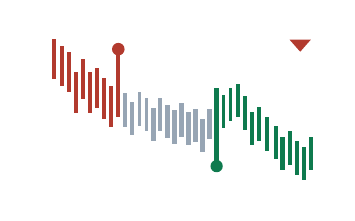
\begin{tikzpicture}[x=0.21839mm,y=0.21839mm]\useasboundingbox (0,0) rectangle (174.0,96.0);\chartssmini\end{tikzpicture}\par\vspace{2.4mm}
{\color{sell}\bfseries\lbl SELL STOP}
\end{minipage}
\par\vspace{14mm}
\begin{tabular}{@{}p{32mm}p{34mm}p{30mm}p{16mm}p{40mm}@{}}
\hd{Type} & \hd{At price liegt} & \hd{Auslöser} & \hd{Dann} & \hd{Take-Profit liegt} \\
\addlinespace[1.6mm]\midrule \addlinespace[2.4mm]
\textcolor{buy}{\bfseries BUY LIMIT} & unter dem Kurs & Kurs fällt & BUY & \textbf{über} dem At price \\ \addlinespace[2mm]
\textcolor{sell}{\bfseries SELL LIMIT} & über dem Kurs & Kurs steigt & SELL & \textbf{unter} dem At price \\ \addlinespace[2mm]
\textcolor{buy}{\bfseries BUY STOP} & über dem Kurs & Kurs steigt & BUY & \textbf{über} dem At price \\ \addlinespace[2mm]
\textcolor{sell}{\bfseries SELL STOP} & unter dem Kurs & Kurs fällt & SELL & \textbf{unter} dem At price \\ \addlinespace[2mm]
\end{tabular}
\begin{merk}\textbf{Drei Faustregeln.} Erst die Richtung – Buy oder Sell. Dann der Ort –
At price über oder unter dem aktuellen Kurs. Aus beidem ergibt sich der Ordertyp von selbst.
Zweitens: Limit wartet auf den besseren Kurs, Stop wartet auf die Bewegung. Drittens: der
\textbf{Take-Profit} liegt immer dort, wo dein Gewinn entsteht – bei einem \textbf{Buy}
über dem At price, bei einem \textbf{Sell} darunter.\end{merk}
\clearpage
\kicker{}{In der Plattform}
\Hone{Der Reiter „New Pending Order“}
\begin{minipage}{125mm}\lead{Links das Fenster, rechts die fünf Stellen,
auf die es ankommt. Alles andere kannst du fürs Erste ignorieren.}\end{minipage}
\par\vspace{9mm}
\noindent\begin{minipage}[t]{80mm}\vspace{0pt}
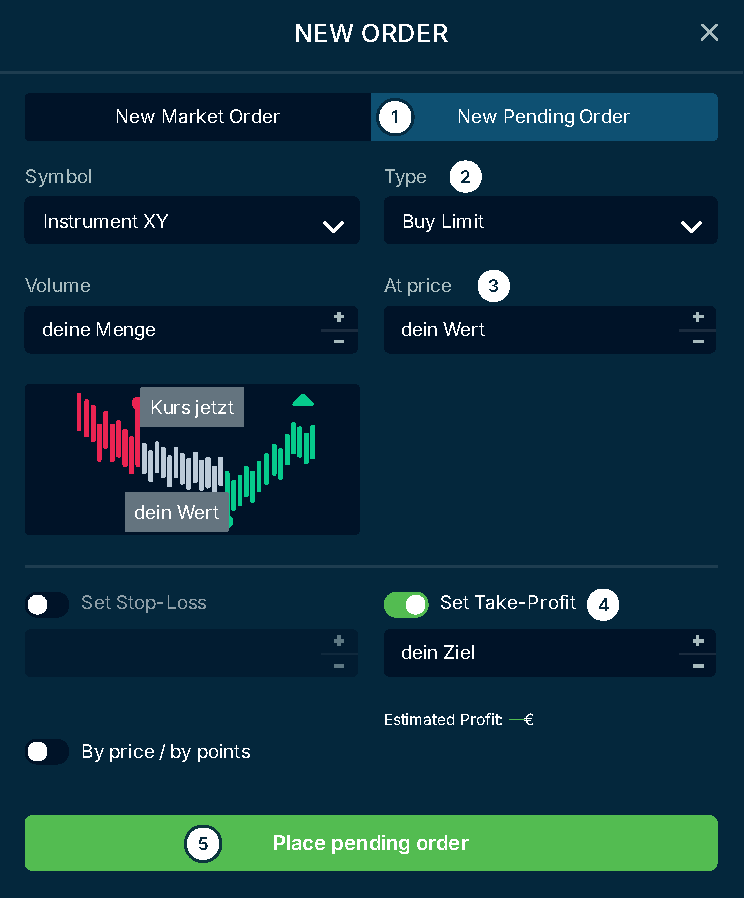
\includegraphics[width=80mm]{fenster-bl.pdf}\end{minipage}\hfill
\begin{minipage}[t]{83mm}\vspace{-1mm}\raggedright
\begin{enumerate}[label=\protect\cn{\arabic*},leftmargin=7mm,labelsep=3mm,itemsep=4.2mm,topsep=0pt]
\item {\bfseries New Pending Order}\newline{\color{muted}\small Der linke Reiter kauft oder verkauft sofort.
Nur rechts kannst du einen Aktivierungspunkt eintragen, auf den gewartet wird.}
\item {\bfseries Type}\newline{\color{muted}\small Deine vier Möglichkeiten: Buy Limit, Sell Limit,
Buy Stop, Sell Stop.}
\item {\bfseries At price}\newline{\color{muted}\small Dein Aktivierungspunkt: der Wert, bei dem
die Pending Order ausgelöst wird. Bei Buy Limit gehört er unter den aktuellen Kurs.}
\item {\bfseries Set Take-Profit}\newline{\color{muted}\small Dein Gewinnziel. Darunter rechnet
die Plattform aus, was dabei herauskäme.}
\item {\bfseries Place pending order}\newline{\color{muted}\small Absenden. Ab jetzt wartet die
Order, bis der Kurs deinen At-price-Wert berührt.}
\end{enumerate}\end{minipage}
\hr
\Htwo{Das Type-Menü und die Regel dahinter}
\noindent\begin{minipage}[t]{46mm}\vspace{0pt}
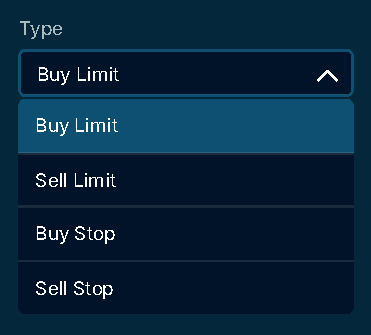
\includegraphics[width=46mm]{type-menu.pdf}\par\vspace{2.5mm}
{\color{soft}\lbl Klick auf \textbf{Type} öffnet genau diese vier.}
\end{minipage}\hfill
\begin{minipage}[t]{118mm}\vspace{0pt}
\begin{prule}{buy}\textbf{BUY LIMIT}\hfill At price {\bfseries unter} dem Kurs\qquad Take-Profit {\bfseries über} At price\end{prule}
\begin{prule}{sell}\textbf{SELL LIMIT}\hfill At price {\bfseries über} dem Kurs\qquad Take-Profit {\bfseries unter} At price\end{prule}
\begin{prule}{buy}\textbf{BUY STOP}\hfill At price {\bfseries über} dem Kurs\qquad Take-Profit {\bfseries über} At price\end{prule}
\begin{prule}{sell}\textbf{SELL STOP}\hfill At price {\bfseries unter} dem Kurs\qquad Take-Profit {\bfseries unter} At price\end{prule}
\end{minipage}
\par\vspace{3.5mm}{\color{muted}\small Passt der Wert nicht zur Regel, bleibt der grüne Button
gesperrt. Beim Wechsel des Ordertyps füllt die Plattform ihn automatisch in die passende Richtung vor –
prüfe ihn trotzdem.}
\begin{merk}\textbf{Der Ablauf in einem Satz.} Du wählst unter \textbf{Type} eine der vier Möglichkeiten, trägst bei
\textbf{At price} deinen Aktivierungspunkt ein, und setzt bei
\textbf{Set Take-Profit} dein Ziel. Danach wartet die Order, bis der Kurs deinen Wert
berührt – und erst dann wird gekauft oder verkauft.\end{merk}

\end{document}
